\documentclass[../thesis.tex]{subfiles}

\begin{document}

\section{JavaScript}
\subfile{./javascript.tex}

\section{Node.js}

Το Node.js είναι ένα open-source runtime environment για την JavaScript.
Δημιουργήθηκε το 2009 από τον Ryan Dahl με στόχο τη δυνατότητα εκτέλεσης αποδοτικών προγραμμάτων υψηλού ταυτοχρονισμού (high concurrency) βασιζόμενη σε μία event-driven και non-blocking αρχιτεκτονική.
Η κύρια χρήση του Node.js είναι ως περιβάλλον για την εκτέλεση backend εφαρμογών, δηλαδή για τη λειτουργία ενός server.

Μέσω του Node.js ο Ryan Dahl θέλησε να δώσει λύση σε ένα πρόβλημα που ήταν μέχρι τότε διαδεδομένο στον τομέα των εφαρμογών server, αυτό της αδυναμίας διαχείρισης μεγάλου όγκου ταυτόχρονων συνδέσεων.
Η δομή των περισσότερων εφαρμογών server βασιζόταν στην αυστηρά σειριακή εκτέλεση εντολών και στη χρήση πολλών ξεχωριστών threads για την εξυπηρέτηση όλων των συνδέσεων, επομένως η απαιτήσεις πόρων και το latency ήταν ιδιαίτερα αυξημένα για εφαρμογές μεγάλης κλίμακας.
Η χρήση διαφορετικών threads θεωρούταν απαραίτητη για την αποφυγή παύσης εκτέλεσης της εφαρμογής στην περίπτωση blocking κλήσεων I/O, όπως πρόσβαση στον δίσκο, σε μία βάση δεδομένων, ή στο διαδίκτυο.
Το Node.js κατάφερε να ξεπεράσει αυτό το εμπόδιο και αξιοποιώντας \textit{non-blocking} κλήσεις I/O και το λεγόμενο \textit{event loop} επιτρέπει την δημιουργία γρήγορων εφαρμογών διαδικτύου που λειτουργούν με ένα μόνο thread.

\begin{figure}[!ht]
    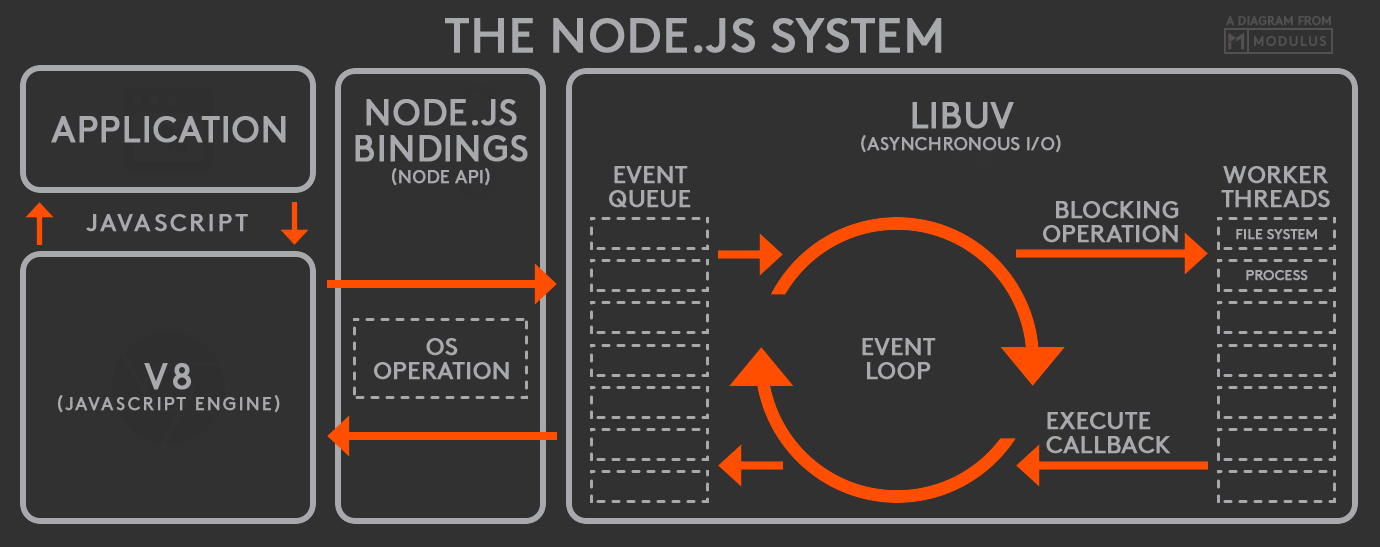
\includegraphics[width=\textwidth]{nodejs_architecture.png}
    \centering
    \caption{Η βασική αρχιτεκτονική του Node.js\cite{node_architecture_diagram}.}
\end{figure}

Ο κεντρικός άξονας του Node.js είναι το event loop.
Το event loop είναι ο βρόχος ο οποίος εκτελείται από το πρόγραμμα καθ' όλη τη διάρκειά ζωής του και είναι υπεύθυνος για την δρομολόγηση των ασύγχρονων λειτουργιών.
Το event loop δέχεται όλα τα σχετικά events που εμφανίζονται (πχ. HTTP requests, callbacks), τα επεξεργάζεται είτε αναθέτοντάς τα στο λειτουργικό σύστημα είτε μέσω ενός thread pool, και έπειτα επιστρέφει στην κανονική ροή του προγράμματος\cite{node_docs_eventloop}. 
Το γεγονός ότι το Node.js αναθέτει τις εργασίες αυτές στο kernel του συστήματος σημαίνει ότι το ίδιο είναι ελεύθερο να συνεχίσει να επεξεργάζεται τα εισερχόμενα events και να εκτελεί τις σύγχρονες διεργασίες, χωρίς να χρειάζεται να περιμένει την ολοκλήρωση των blocking διεργασιών.
Αυτό, σε συνδυασμό με τη single-threaded φύση του event loop, επιτρέπει στο Node.js να χειρίζεται πολύ μεγαλύτερο αριθμό ταυτόχρονων συνδέσεων από άλλες υλοποιήσεις (όπως έναν κλασσικό PHP server), με λιγότερες απαιτήσεις σε μνήμη.
Ο μηχανισμός του event loop αλλά και όλες οι non-blocking λειτουργίες του Node.js, πχ. το network και file I/O, παρέχονται από τη βιβλιοθήκη \texttt{libuv}.
Παρόλο που ο κώδικας JavaScript της εφαρμογή είναι single-threaded, το Node.js αξιοποιεί πολλαπλά threads στο παρασκήνιο για τις παραπάνω λειτουργίες.

\begin{figure}[!ht]
    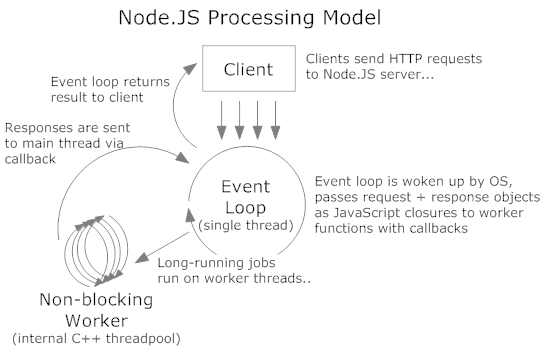
\includegraphics[width=\textwidth]{nodejs_event_loop.png}
    \centering
    \caption{Η λειτουργία του event loop στο Node.js\cite{node_eventloop_diagram}.}
\end{figure}


Προκειμένου να εκτελέσει τον κώδικα JavaScript εκτός του περιβάλλοντος ενός browser, το Node.js χρησιμοποιεί τον V8 engine της Google.

Ο κώδικας που εκτελεί το Node.js είναι κώδικας JavaScript.
Η JavaScript επιλέχθηκε ως η γλώσσα εκτέλεσης όχι μόνο γιατί ήταν ήδη διαδεδομένη στον χώρο των διαδικτυακών εφαρμογών, αλλά κυρίως γιατί είναι κατάλληλα σχεδιασμένη για να υποστηρίξει τις απαιτήσεις τους Node.js.
Από την απαρχή της η JavaScript υποστήριζε τον event-driven και ασύγχρονο προγραμματισμό, καθώς αυτός ήταν απαραίτητος για την ομαλή non-blocking λειτουργία των ιστοσελίδων, ενώ οι ανώνυμες συναρτήσεις και τα function closures ευνοούσαν περαιτέρω τη χρήση των callbacks.
Η χρήση της JavaScript στο Node.js δίνει επίσης τη δυνατότητα για full-stack JavaScript development, δηλαδή ομοιόμορφη χρήση της JavaScript για την ανάπτυξη τόσο του frontend όσο και του backend μέρους μίας εφαρμογής.

Το Node.js άρχισε να γίνεται διάσημο σύντομα μετά από την παρουσίασή του, και πλέον η πλειοψηφία όλων των εταιριών παγκοσμίως χρησιμοποιούν το Node.js σε κάποιο τουλάχιστον μέρος του backend τους.
Κάποιες εταιρίες που χρησιμοποιούν σε μεγάλο βαθμό το Node.js είναι η Netflix\cite{netflix}, η PayPal\cite{paypal}, η LinkedIn\cite{linkedIn}, η NASA\cite{nasa}, και η Bloomberg\cite{bloomberg}.
Στο παρελθόν η Uber επίσης χρησιμοποιούσε το Node.js για το μεγαλύτερο μέρος του backend της, και μάλιστα ήταν από τις πρώτες μεγάλες εταιρίες που το υιοθέτησαν\cite{uberNode}.

\end{document}